\begin{enumerate}[label=\thechapter.\arabic*,ref=\thechapter.\theenumi]
\item Consider the signals $x\brak{n}$=$2^{n-1} u\brak{ -n+2}$ and $y\brak{n}$=$2^{-n+2}u\brak{ n+1}$, where $u\brak{n}$ is the unit step sequence. Let $X\brak{e^{j\omega}}$ and $Y\brak{e^{j\omega}}$ be the discrete-time Fourier of $x\brak{n}$ and $y\brak{n}$,respectively. The value of the integral $\frac{1}{2\pi}\int_{0}^{2\pi} X\brak{e^{j\omega}} Y\brak{e^{-j\omega}} d \omega$
(rounded off to one decimal place) is \underline{{\hspace{1.5in}}}\\
\hfill{(GATE EC 41 2021)}\\
\solution

\let\negmedspace\undefined
\let\negthickspace\undefined
\documentclass[journal,12pt,twocolumn]{IEEEtran}
\usepackage{cite}
\usepackage{amsmath,amssymb,amsfonts,amsthm}
\usepackage{algorithmic}
\usepackage{graphicx}
\usepackage{textcomp}
\usepackage{xcolor}
\usepackage{txfonts}
\usepackage{listings}
\usepackage{enumitem}
\usepackage{mathtools}
\usepackage{gensymb}
\usepackage{comment}
\usepackage[breaklinks=true]{hyperref}
\usepackage{tkz-euclide} 
\usepackage{listings}
\usepackage{gvv}                                        
\def\inputGnumericTable{}                                 
\usepackage[latin1]{inputenc}                                
\usepackage{color}                                            
\usepackage{array}                                            
\usepackage{longtable}                                       
\usepackage{calc}                                             
\usepackage{multirow}                                         
\usepackage{hhline}                                           
\usepackage{ifthen}                                           
\usepackage{lscape}

\newtheorem{theorem}{Theorem}[section]
\newtheorem{problem}{Problem}
\newtheorem{proposition}{Proposition}[section]
\newtheorem{lemma}{Lemma}[section]
\newtheorem{corollary}[theorem]{Corollary}
\newtheorem{example}{Example}[section]
\newtheorem{definition}[problem]{Definition}
\newcommand{\BEQA}{\begin{eqnarray}}
\newcommand{\EEQA}{\end{eqnarray}}
\newcommand{\define}{\stackrel{\triangle}{=}}
\theoremstyle{remark}
\newtheorem{rem}{Remark}
\begin{document}
\bibliographystyle{IEEEtran}
\vspace{3cm}
\title{\textbf{EC-2021}}
\author{EE23BTECH11210-Dhyana Teja Machineni$^{*}$% <-this % stops a space
}
\maketitle
\newpage
\bigskip

\textbf{QUESTION:}\\
Consider the signals $x\brak{n}$=$2^{n-1} u\brak{ -n+2}$ and $y\brak{n}$=$2^{-n+2}u\brak{ n+1}$, where $u\brak{n}$ is the unit step sequence. Let $X\brak{e^{j\omega}}$ and $Y\brak{e^{j\omega}}$ be the discrete-time Fourier of $x\brak{n}$ and $y\brak{n}$,respectively. The value of the integral $\frac{1}{2\pi}\int_{0}^{2\pi} X\brak{e^{j\omega}} Y\brak{e^{-j\omega}} d \omega$
(rounded off to one decimal place) is \underline{{\hspace{1.5in}}}\\
\hfill{(GATE EC 41 2021)}\\

\solution\\

\begin{table}[h]
         
\begin{tabular}{|c|c|l|}
\hline
Parameter  & Value & Description   \\             
\hline
$y(0)$     & $0$   & Initial displacement  \\     
 \hline
$y'(0)$    & $0$   & First derivative at $t=0$  \\
 \hline
$y''(0)$   & $0$   & Second derivative at $t=0$ \\
 \hline
$y'''(0)$  & $0$   & Third derivative at $t=0$  \\
 \hline
\end{tabular}


         \caption{Variables and their descriptions}
     \end{table}
\begin{align}
    V&=\frac{1}{2\pi}\int_{0}^{2\pi} X\brak{e^{j\omega}} Y\brak{e^{-j\omega}} d \omega\\
     Z\brak{e^{j\omega}}&= X\brak{e^{j\omega}} Y\brak{e^{-j \omega}}\\
           z(n)&\xrightarrow{\mathcal{F}} Z(e^{j\omega})\\
           z\brak{n}&=\frac{1}{2\pi}\int_{-\pi}^{\pi} Z\brak{e^{j\omega}} e^{j\omega n} d\omega\\
      z\brak{0}&=\frac{1}{2\pi}\int_{0}^{2\pi} Z\brak{e^{j\omega}} d \omega\\
   z\brak{ n}&= x\brak{n} * y\brak{-n}\\
   &=\sum_{k=-\infty}^{\infty} 2^{k-1} u\brak{-k+2} 2^{n-k+2} u\brak{-n+k+1}\\
   &=\sum_{k=-\infty}^{2} 2^{n+1} u\brak{k-n+1}\\
   z(0)&=\sum_{k=-\infty}^{2} 2 u\brak{k+1}\\
   &=2\sum_{k=-1}^{2}u\brak{k+1}\\
  \therefore z\brak{0} &=8
\end{align}
$\therefore$ $\frac{1}{2\pi}\int_{0}^{2\pi} X\brak{e^{j\omega}} Y\brak{e^{-j\omega}} d \omega$= $8$
\renewcommand{\thefigure}{\theenumi}
 \renewcommand{\thetable}{\theenumi}
\begin{figure}[h]
  
  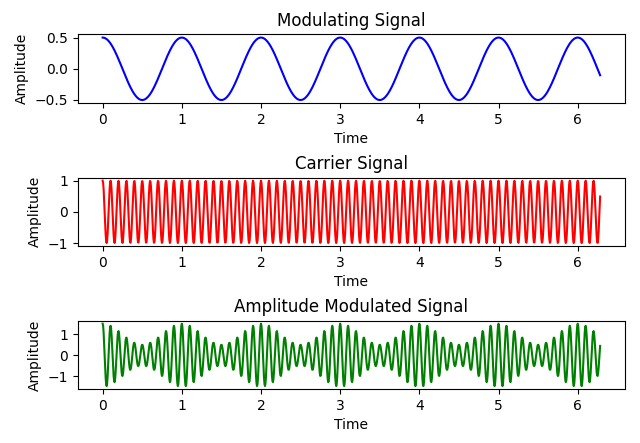
\includegraphics[width=\columnwidth]{figs/Figure_1.png}
  \caption{Stem Plot of $z\brak{n}$}
\end{figure}
\end{document}

\pagebreak
\item Given that $\mathcal{S}$ is the unit circle in the counter clock-wise direction with its centre at origin, the integral
        $\oint \brak{\frac{z^3}{4z-\jmath}}dz=\rule{1cm}{0.15mm}$
 (round off to theree decimal places)
 \hfill{(GATE 2022 AE)}\\
 \solution\\
 


\end{enumerate}
